\documentclass[11pt]{article}
%you can look for fun LaTeX packages to use hereasdf

\usepackage{amsmath}
\usepackage{amssymb}
\usepackage{fancyhdr}
\usepackage{amsthm}

\usepackage{graphicx}
\usepackage{dcolumn}
\usepackage{bm}

%fun commands for fun sets
%make sure to use these in math mode
\newcommand{\Z}{\mathbb{Z}}
\newcommand{\R}{\mathbb{R}}
\newcommand{\N}{\mathbb{N}}
\newcommand{\C}{\mathbb{C}}
\newcommand{\m}{\mathcal{M}}
\newcommand{\Tt}{\mathcal{T}}
\newcommand{\pa}{\partial}
\newcommand{\dD}{\mathcal{D}}
\newcommand{\E}{\mathbb{E}}



\oddsidemargin0cm
\topmargin-2cm    
\textwidth16.5cm   
\textheight23.5cm  

\newcommand{\question}[2] {\vspace{.25in} \hrule\vspace{0.5em}
\noindent{\bf #1: #2} \vspace{0.5em}
\hrule \vspace{.10in}}
\renewcommand{\part}[1] {\vspace{.10in} {\bf (#1)}}

\newcommand{\myname}{Alex Havrilla}
\newcommand{\myandrew}{alumhavr}
\newcommand{\myhwnum}{Hw 1}

\newtheorem{theorem}{Theorem}
\newtheorem{prop}{Prop}
\theoremstyle{remark}
\newtheorem{lemma}{Lemma}
\newtheorem{remark}{Remark}
\newtheorem{defi}{Def}
\newtheorem{apps}{Application}
\newtheorem{quest}{Question}
\newtheorem{ans}{Answer}
\newtheorem{interest}{Interesting}
\newtheorem{theme}{Theme}
\newtheorem{back}{Background}
\newtheorem{idea}{Idea}
\newtheorem{example}{Example}

\setlength{\parindent}{0pt}
\setlength{\parskip}{5pt plus 1pt}
 
\pagestyle{fancyplain}
\lhead{\fancyplain{}{\textbf{HW\myhwnum}}}      % Note the different brackets!
\rhead{\fancyplain{}{\myname\\ \myandrew}}
\chead{\fancyplain{}{\mycourse}}

\linespread{1.3}

\title{Technical Animation}

\begin{document}

\maketitle

\section{Introductions}

\textbf{TAG:} TechnicalAnimation

\begin{interest}
	TA Arjun is interested in PDEs and numerical simulation.
\end{interest}

\begin{remark}
	Course Website:
	\begin{verbatim}
		http://graphics.cs.cmu.edu/nsp/course/15464-s21/www/
	\end{verbatim}

	\textit{Computer Animation: Algorithms and Techniques} is the course textbook. In drive.
\end{remark}

\begin{quest}
	Does greater physical simulation accuarcy lead to a less palatable viewing experience? 
\end{quest}

\begin{ans}
	Not sure but often directors will personify animations and we have different parameters to give differenter personfications. For example "angry storm".
\end{ans}

\begin{ans}
	It seems exaggerated motion is often more digestestible(think actors for example). Often used actors in motion capture
\end{ans}

\begin{interest}
	Rig Net: automatically rigging meshes. Note: rigging is process of jointing meshes, providing structure/skeleton.
\end{interest}

\begin{remark}
	Beginning of rigging: find medial axis of geometry and impose some structure.
\end{remark}

\subsection{Examples in Practice}

\textbf{TAG:} TechnicalAnimation

\begin{remark}
	L-systems developed to describe plant structures and generation.
\end{remark}

\begin{remark}
	Tools for good animation: The Anmimators Survival Kit.
\end{remark}

\begin{remark}
	Idea behind rigging: for easy animating want ball control points you can manipulate for convenience.
\end{remark}

\begin{remark}
	Cloth simulation involves a mesh...
	Cloth intersection problems in Pixar's Coco:
	\begin{verbatim}
		https://www.researchgate.net/publication/326907399_Better_collisions_and_faster_cloth_for_Pixar's_Coco
	\end{verbatim}
\end{remark}

\begin{remark}
	Traditional animation: keyframing. 

	New variant: procedural animation. Often used for crowd animation.
\end{remark}

\begin{interest}
	Interesting site:
	\begin{verbatim}
	www.massivesoftware.com
	\end{verbatim}
\end{interest}

\begin{interest}
	Character controller using Motion VAEs interesting.
\end{interest}

\subsection{2/8}

\begin{remark}
	3 techniques for animation: motion capture, procedural, and keyframing.
\end{remark}

\begin{remark}
	CMU Panoptic Studio Dataset: Mocap data
\end{remark}

\begin{remark}
	Motion Capture Data Explained
\end{remark}



\section{Inverse Kinematics}

\textbf{TAG:} TechnicalAnimation InverseKinematics

\begin{remark}
	CCD Illustration:
	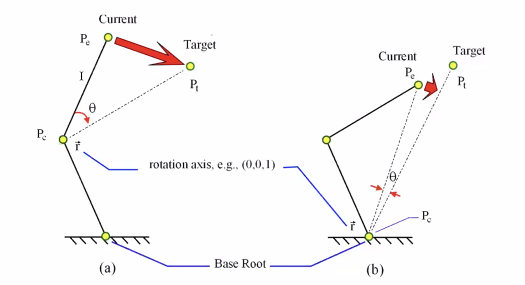
\includegraphics[width=250px]{C:/Users/Alex/Desktop/Notes/Spring 2021/pics/ccd.png}
\end{remark}

\begin{remark}
	Long chains of links tend to wrap up. Can also decide to iterate top to bottom affector or bottom to top. To address this can repeat recursion for every top level: whatever gets recursed more seems to bend more.
\end{remark}

\begin{remark}
	Basic model/fast but some limitations. Fabric better repacement
\end{remark}


\begin{remark}
	Alternative approach is jacobian based inverse kinematics: Introduction to Invers Kinematics with Jacobian Transpose, Pseudoinverse and Damped Leaster Squares
	\begin{verbatim}
		http://math.ucsd.edu/~sbuss/ResearchWeb/ikmethods/iksurvey.pdf
	\end{verbatim}
\end{remark}

\begin{remark}
	We write jacobian as:
	\begin{align*}
		\dot{s} = J(\theta)\dot{\theta}
	\end{align*}

	for speeds on the affectors and their bending angles as we move to a target point. Ie. the change in $s$(position of end affector) against the change in angles.
\end{remark}

\begin{prop}
	\begin{align*}
		\frac{\partial s}{\partial \theta_j} = v_j \times (s - p_j)
	\end{align*}
	where $v_j$ is the axis of rotation for each joint. We take the cross product of line from joint to end affector and rotation axis to get the direction of movement due to that joint(think single arm rotating around line gives tangent to the line)
\end{prop}

\begin{remark}
	To solve $\dot{s} = J\dot{\theta}$ would just want to take inverse but not always possible obviously
\end{remark}

\begin{remark}
	The jacobian transpose always at least does not move away from target: $\langle  J J^T e, e \rangle \geq0$. Often less expensive than pseudoinverse $J^{-1}$ method. 
\end{remark}

\begin{remark}
	For pseudoinverse method we get
	\begin{align*}
		\Delta\theta = J^T(JJ^T)^{-1}e
	\end{align*}
	Note e is $\Delta s$
\end{remark}

\begin{remark}
	Anoter option is damped least squares(really l2 regression). Then
	\begin{align*}
		\Delta \theta = J^T(JJ^T + \lambda^2I)^{-1}e
	\end{align*}

	which we know will be invertible

	Can be solved with line search(grid search) or other techniques
\end{remark}

\begin{remark}
	Example: Want robot hand with 24 degrees of freedom to hit 10 points. So highly underconstrained and thus was resulting in weird, nonnatural solutions. Use Nullspace technique to add some constraint.
	\begin{align*}
		\Delta \theta = J^+e+ (I-J^+J)\phi
	\end{align*}

	want to damp inner joints without affecting result on end affector
\end{remark}


\end{document}

